\documentclass[fleqn,10pt,a4paper]{article}
\usepackage{polski}
\usepackage[T1]{fontenc}
\usepackage[utf8]{inputenc}
\usepackage[a4paper, left=2.5cm, right=2.5cm, top=2.5cm, bottom=2.5cm]{geometry} 
\usepackage{enumerate}
\usepackage{sidecap}
\usepackage{wrapfig}
\usepackage{subfig}
\usepackage{fancyhdr}
\usepackage{multirow}
\usepackage{gensymb}
\usepackage{graphicx}
\usepackage{url}
\usepackage{xurl}
\usepackage{hyperref}
\usepackage{array}
\usepackage{amsmath}
\usepackage{textcomp}
\usepackage{verbatim}
\usepackage{media9}
\usepackage{listings}
\usepackage{color}
\usepackage{listings}
\usepackage{color}

\definecolor{mygreen}{rgb}{0,0.6,0}
\definecolor{mygray}{rgb}{0.5,0.5,0.5}
\definecolor{mymauve}{rgb}{0.58,0,0.82}

\lstset{
  language=Python,
  basicstyle=\footnotesize\ttfamily,
  commentstyle=\color{mygreen},
  keywordstyle=\color{blue},
  numberstyle=\tiny\color{mygray},
  numbers=none,
  stringstyle=\color{mymauve},
  breaklines=true,
  showstringspaces=false,
  frame=single,
  backgroundcolor=\color{white},
  literate={ą}{{\k{a}}}1 {ć}{{\'c}}1 {ę}{{\k{e}}}1 {ł}{{\l}}1 {ń}{{\'n}}1 {ó}{{\'o}}1 {ś}{{\'s}}1 {ź}{{\'z}}1 {ż}{{\.z}}1
}

\hypersetup{
  colorlinks=true,
  linkcolor=black,
  filecolor=magenta,      
  urlcolor=cyan,
}

\hypersetup{breaklinks=true}
\urlstyle{same}
\renewcommand{\lstlistingname}{Kod źródłowy}
\renewcommand{\lstlistlistingname}{Spis kodów źródłowych}
\renewcommand{\figurename}{Wykres}

\makeatletter
\renewcommand{\maketitle}{%
  \begin{titlepage}
    \begin{center}
      \vspace*{2cm}
      {\huge \@title \par}
      \vspace{1.5cm}
      {\large \@author \\ 325693 \par}
      {\large Wydział Geodezji i Kartografii\\ Politechnika Warszawska \par}
      \vspace{1.5cm}
      {\large Dane nr 15 - FK5 899 \par}
      {\large $\alpha = 23h \, 55m \,34.219s$ \\ $\delta = 57 \degree \, 37' \, 48.71''$\par}
      \vspace{9cm}
      {\large \@date \par}
      \vspace{1.5cm}
    \end{center}
  \end{titlepage}
}
\makeatother
    \title{\textbf{SPRAWOZDANIE Z ĆWICZENIA 1:}\\ Transformacja współrzędnych gwiazdy z układu równikowego do horyzontalnego}
\author{Maja Kret}
\date{Warszawa, \today}


\setlength{\parindent}{0cm}
\setlength{\parskip}{1ex plus 0.5ex minus 0.2ex}
\linespread{1.3}


\begin{document} 
\pagestyle{fancy}
\fancyhf{}
\rfoot{\thepage}
\renewcommand{\headrulewidth}{0pt}
\maketitle
\rhead{~}

\tableofcontents
\newpage

\section{Cel ćwiczenia}
Celem ćwiczenia jest transformacja współrzędnych gwiazdy FK5 899 - Ro Cassiopeiae z układu równkowego na horyzontalny
oraz wizualizacja jej położenia z dwóch miejsc obserwacji w ciągu doby 1 lipca 2023.

\section{Wstęp teoretyczny}
\subsection{Układ współrzędnych równikowych ekwinokcjalnych}
Jest to globalny system współrzędnych, niezależny od lokalizacji obserwatora. 
Oparty jest na płaszczyźnie równika niebieskiego i służy do opisu położenia gwiazd na sferze niebieskiej.
W tym układzie, deklinacja $\delta$ jest odpowiednikiem szerokości geograficznej, podczas gdy rektascenzja $\alpha$ odpowiada 
długości geograficznej. Punkt Barana, przez który Słońce przechodzi w dniu równonocy wiosennej, jest używany jako punkt 
odniesienia dla rektascenzji.
\subsection{Układ współrzędnych horyzontalnych}
Układ horyzontalny opiera się na lokalnym położeniu obserwatora. 
Najważniejszym punktem tego układu jest zenit - punkt na nieboskłonie dokładnie nad głową obserwatora. 
Oś horyzontalna, położona prostopadle do osi zenit-nadir, leży w płaszczyźnie horyzontu obserwatora. 
Współrzędne w tym układzie to azymut $A$ oraz wysokość $h$. Azymut jest mierzony wzdłuż horyzontu zgodnie z kierunkiem ruchu 
wskazówek zegara, podczas gdy wysokość mierzona jest od horyzontu do gwiazdy. 
Mimo swojej użyteczności w praktyce obserwacyjnej, układ horyzontalny nie jest odpowiedni do katalogowania gwiazd 
z powodu jego zależności od czasu i miejsca obserwacji.

\section{Dane do ćwiczenia}

\begin{table}[!h]
\centering
\begin{tabular}{|c|*{3}{w{c}{2em}|}*{3}{w{c}{2em}|c|c|c|}}
\hline
    Nazwa & \multicolumn{3}{c|}{$\alpha$} & \multicolumn{3}{c}{$\delta$} & \multicolumn{3}{|c|}{CSE w Warszawie}\\ \hline
    & h & m & s & $^\circ$ & ' & '' & wsch. & górow. & zach. \\ \hline
    FK5 899 & 23 & 55 & 34.219 & 57 & 37 & 48.71 & \multicolumn{3}{c|}{}\\ \hline
    Słońce & 6 & 37 & 43.973 & 23 & 8 & 11.85 & 3:19 && 20:00\\ \hline
    Księżyc & 16 & 9 & 45.978 & -23 & 54 & 48.69 & 18:32 & 22:02 & 0:51 \\ \hline

\end{tabular}
\caption{Współrzędne badanych obiektów z Rocznika Astronomicznego na epokę 2023.5
\label{gwiazda}}
\end{table}

Do danych zostały dodane czasy wschodu, górowania i zachodu Słońca oraz Księżyca w Warszawie.
Powinny one ułatwić interpretację wyników oraz umożliwić sprawdzenie poprawności wykresów.
\clearpage
\begin{table}[!h]
  \centering
  \begin{tabular}{|c|c|*{3}{c|}*{3}{c|}}
    \hline
    Nazwa & Nr w FK5 & \multicolumn{3}{c|}{$\alpha$} & \multicolumn{3}{c|}{$\delta$} \\ \hline
    & & h & m & s & $^\circ$ & ' & '' \\ \hline
    Merak & 416 & 11 & 3 & 14.669 & 56 & 15 & 21.18  \\ \hline
    Dubhe & 417 & 11 & 5 & 9.530 & 61 & 37 & 24.44  \\ \hline
    Phecda & 447 & 11 & 55 & 3.388 & 53 & 33 & 50.55 \\ \hline
    Megrez & 456 & 12 & 16 & 34.755 & 56 & 54 & 7.80  \\ \hline
    Alioth & 483 & 12 & 55 & 3.395 & 55 & 49 & 57.62 \\ \hline
    Mizar & 497 & 13 & 24 & 52.075 & 54 & 48 & 11.50 \\ \hline
    Alkaid & 509 & 13 & 48 & 27.861 & 49 & 11 & 48.04 \\ \hline
  \end{tabular}
  \caption{Współrzędne gwiazd Wielkiego Wozu na epokę 2023.5}
  \label{tab:gwiazda}
\end{table}

\begin {table}[!h]
\centering
\begin{tabular}{|c|c|c|c|} \hline
    & $\varphi$ & $\lambda$ \\ \hline
    Warszawa & 52\degree & 21\degree \\ \hline
    Równik & 0\degree & 21\degree \\ \hline
\end{tabular}
\caption{Współrzędne obserwatora
\label{pozycja}}
\end{table}


\section{Przebieg ćwiczenia}

\begin{enumerate}
  \item \textbf{Konwersja współrzędnych kątowych:}
  Funkcje \texttt{dms2deg} i \texttt{dms2rad} z Kodu źródłowego \ref{kod1} konwertują współrzędne gwiazd z formatu stopnie, minuty, 
  sekundy (mds) na stopnie (deg) oraz radiany (rad).

  \item \textbf{Obliczenie dnia juliańskiego:}
  Funkcja \texttt{julday} z Kodu \ref{kod2} oblicza dzień juliański, co jest konieczne do późniejszego obliczenia 
  Czasu Gwiazdowego (Greenwich Mean Sidereal Time).

  \item \textbf{Obliczenie Czasu Gwiazdowego:}
  Funkcja \texttt{GMST} opisana w Kodzie \ref{kod2} oblicza Czas Gwiazdowy w Greenwich na podstawie dnia juliańskiego i zwraca czas 
  w godzinach. Jest to czas gwiazdowy w punkcie zerowym, czyli w Greenwich. Aby uzyskać czas lokalny,
  tzreba uwzględnić też długość geograficzną obserwatora.

  \item \textbf{Obliczenie współrzędnych horyzontalnych:}
  Funkcja \texttt{horizontal\_coords} zawarta w Kodzie źródłowym \ref{kod2} przelicza współrzędne równikowe (deklinacja $\delta$, rektascensja $\alpha$) 
  na współrzędne horyzontalne (wysokość $h$, azymut $A$), używając czasu gwiazdowego oraz współrzędnych 
  geograficznych obserwatora (szerokość geograficzna $\varphi$, długość geograficzna $\lambda$).
  Wartość azymutu jest dostosowywana w zależności od położenia gwiazdy.
  \begin {flalign*}
  & t = (\text{GMST} \cdot 15 + \lambda - \alpha \cdot 15) \mod 360 \\
  & h = \arcsin(\sin(\delta)\sin(\varphi) + \cos(\delta)\cos(\varphi)\cos(t)) \\
  & A = \arccos\left(\frac{\sin(\delta) - \sin(\varphi)\sin(h)}{\cos(\varphi)\cos(h)}\right) 
  \end {flalign*}
  \item \textbf{Interpolacja danych:}
  Funkcja \texttt{interpolate} z Kodu \ref{kod2} używa funkcji \texttt{make\_interp\_spline} z biblioteki \texttt{scipy} do interpolacji danych o wysokości gwiazdy w ciągu dnia, aby uzyskać płynniejszy wykres.

  \item \textbf{Wizualizacja wyników:}
  Używając biblioteki \texttt{matplotlib}, rysowane są różne wykresy, w tym:
  \begin{itemize}
      \item Sfera Niebieska: 3D wykres przedstawiający ruch gwiazdy i Słońca na sferze niebieskiej.
      \item Skyplot: Wykres polar, pokazujący ruch gwiazdy i Słońca na niebie.
      \item Wykres zależności azymutu od czasu.
      \item Wykres zależności wysokości od czasu z interpolacją.
      \item Panorama nieba: Wykres azymutu w funkcji wysokości.
  \end{itemize}
  Ich implementacje dla gwiazdy FK5 899 znajdują się w Kodzie źródłowym \ref{kod4}.

\end{enumerate}

\section{Warszawa}
\subsection{Ro Cassiopeiae i Słońce}
\begin{figure}[h!]
    \centering
    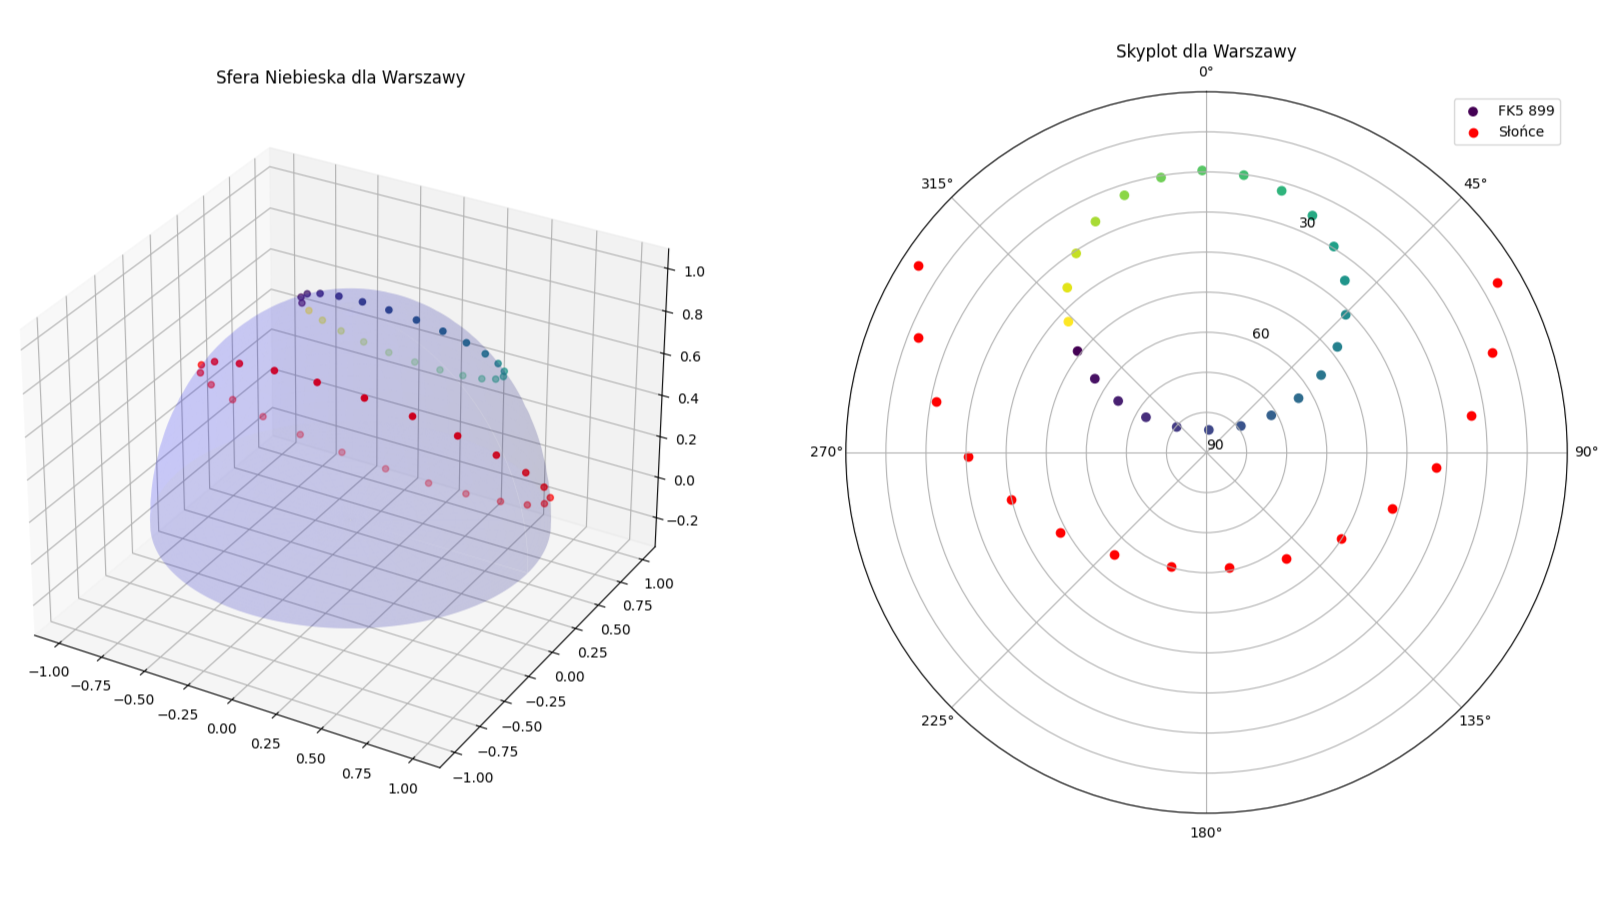
\includegraphics[width=1\textwidth]{zdjecia/fig1_wwa.png}
    \caption{Położenia gwiazd w ciągu doby z punktu obserwacji Warszawa}
    \label{all_wwa}
\end{figure}

Z wykresu \ref{all_wwa} wynika, że gwiazda 899 jest widoczna przez całą dobę i nigdy nie zachodzi. Nie przechodzi też
przez pierwszy wertykał. Słońce natomiast jest widoczne nad horyzontem aż 16h.

Do utworzenia wykresów wysokości \ref{h_wwa} oraz \ref{h_r} została użyta interpolacja, aby lepiej zobrazować faktyczne położenie gwiazd w ciągu doby.

\begin{figure}[h!]
  \centering
  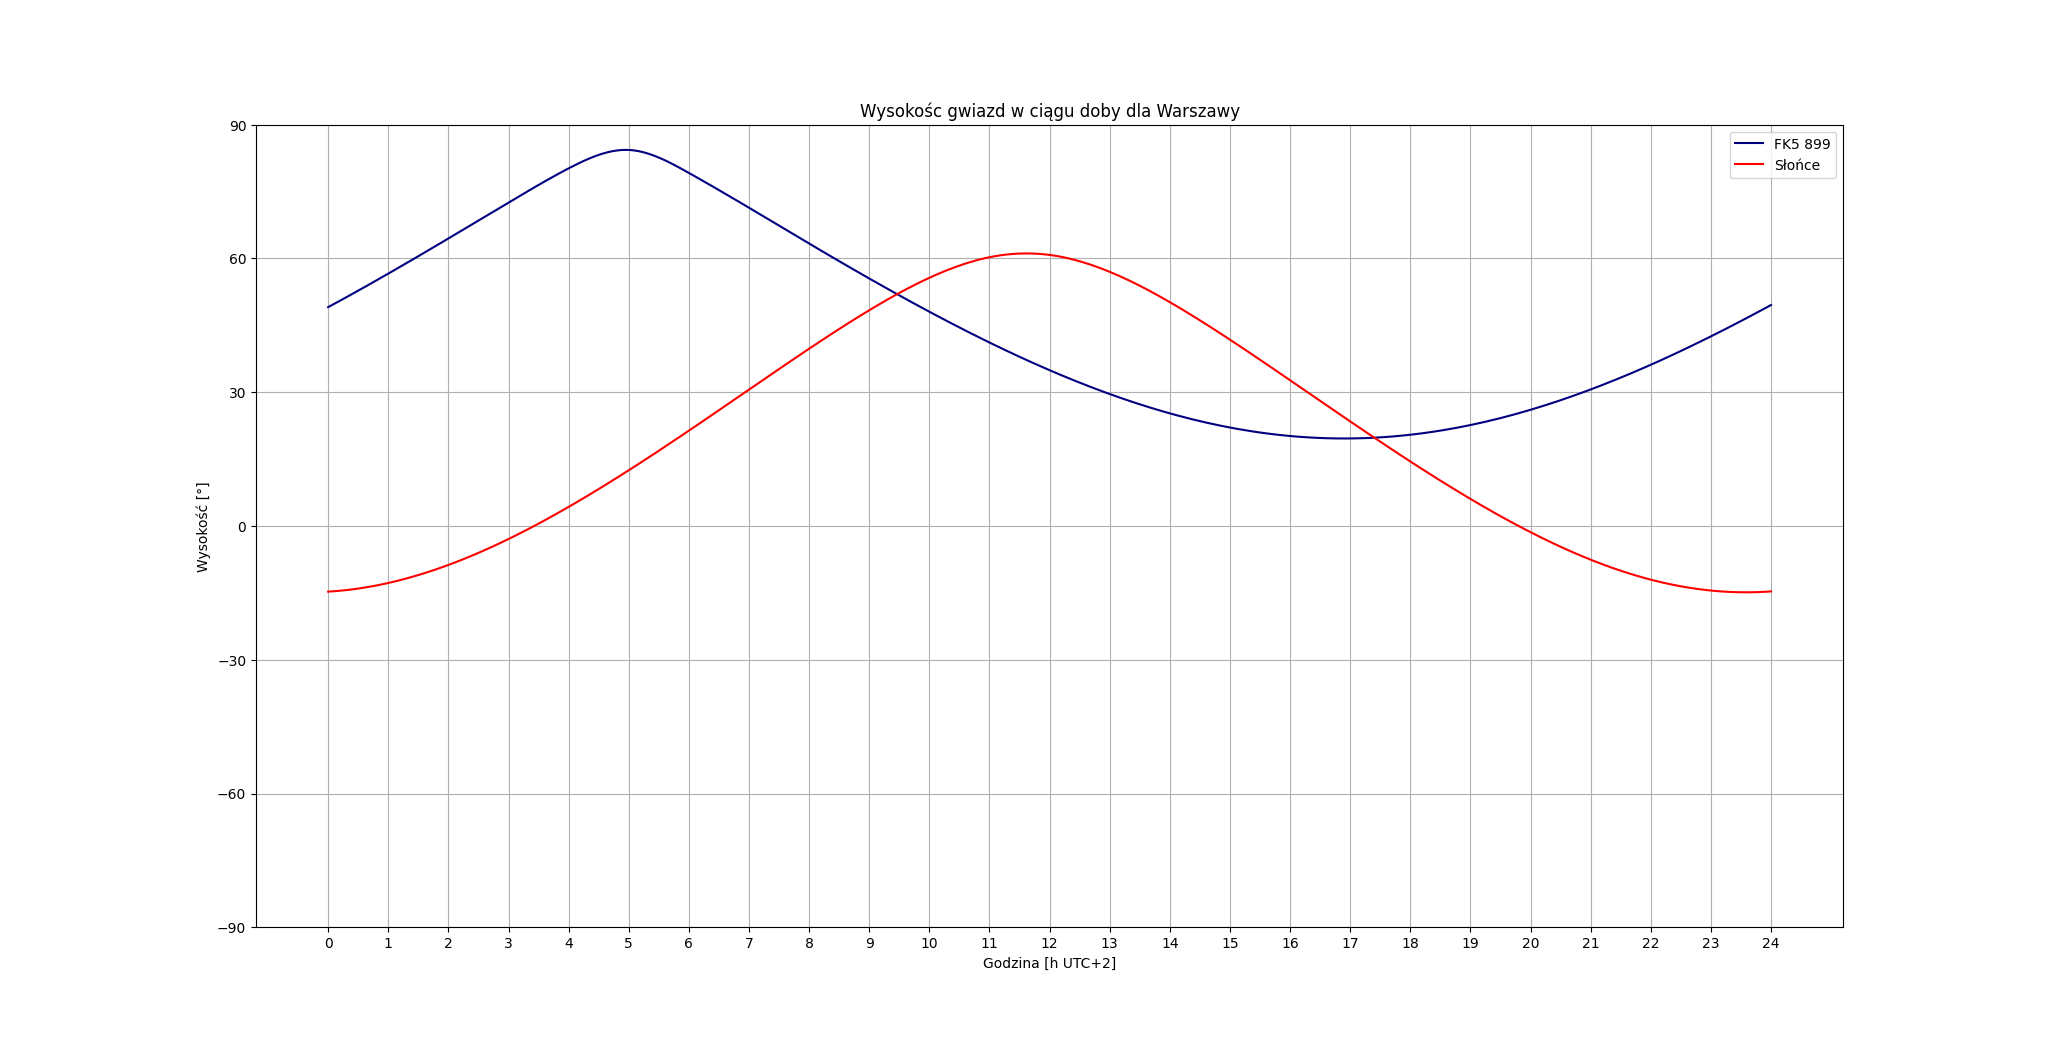
\includegraphics[width=1\textwidth]{zdjecia/wys_gwiazd_wwa_inter.png}
  \caption{Wykres wysokości gwiazd od godziny z punktu obserwacji Warszawa}
  \label{h_wwa}
\end{figure}


Gwiazda 899 pozostaje na wykresie \ref{h_wwa} powyżej 0° wysokości przez całą dobę, co potwierdza, że nie zachodzi poniżej horyzontu.
Jej górowanie można odczytać - jest to około godziny 5:00.

Z wykresu \ref{h_wwa} położenia Słońca można odczytać przybliżone godziny wschodu i zachodu. Wartości te zgadzają się z danymi 
podanymi w Roczniku Astronomicznym na dzień 1 lipca 2023 - wschód o 3:19 i zachód o 20:00. Górowanie z Słońca przypada w okolicach
godziny 12:00, co jest zgodne z oczekiwaniami. Osiąga ono wtedy wysokość około 60°.


\begin{figure}[h!]
  \centering
  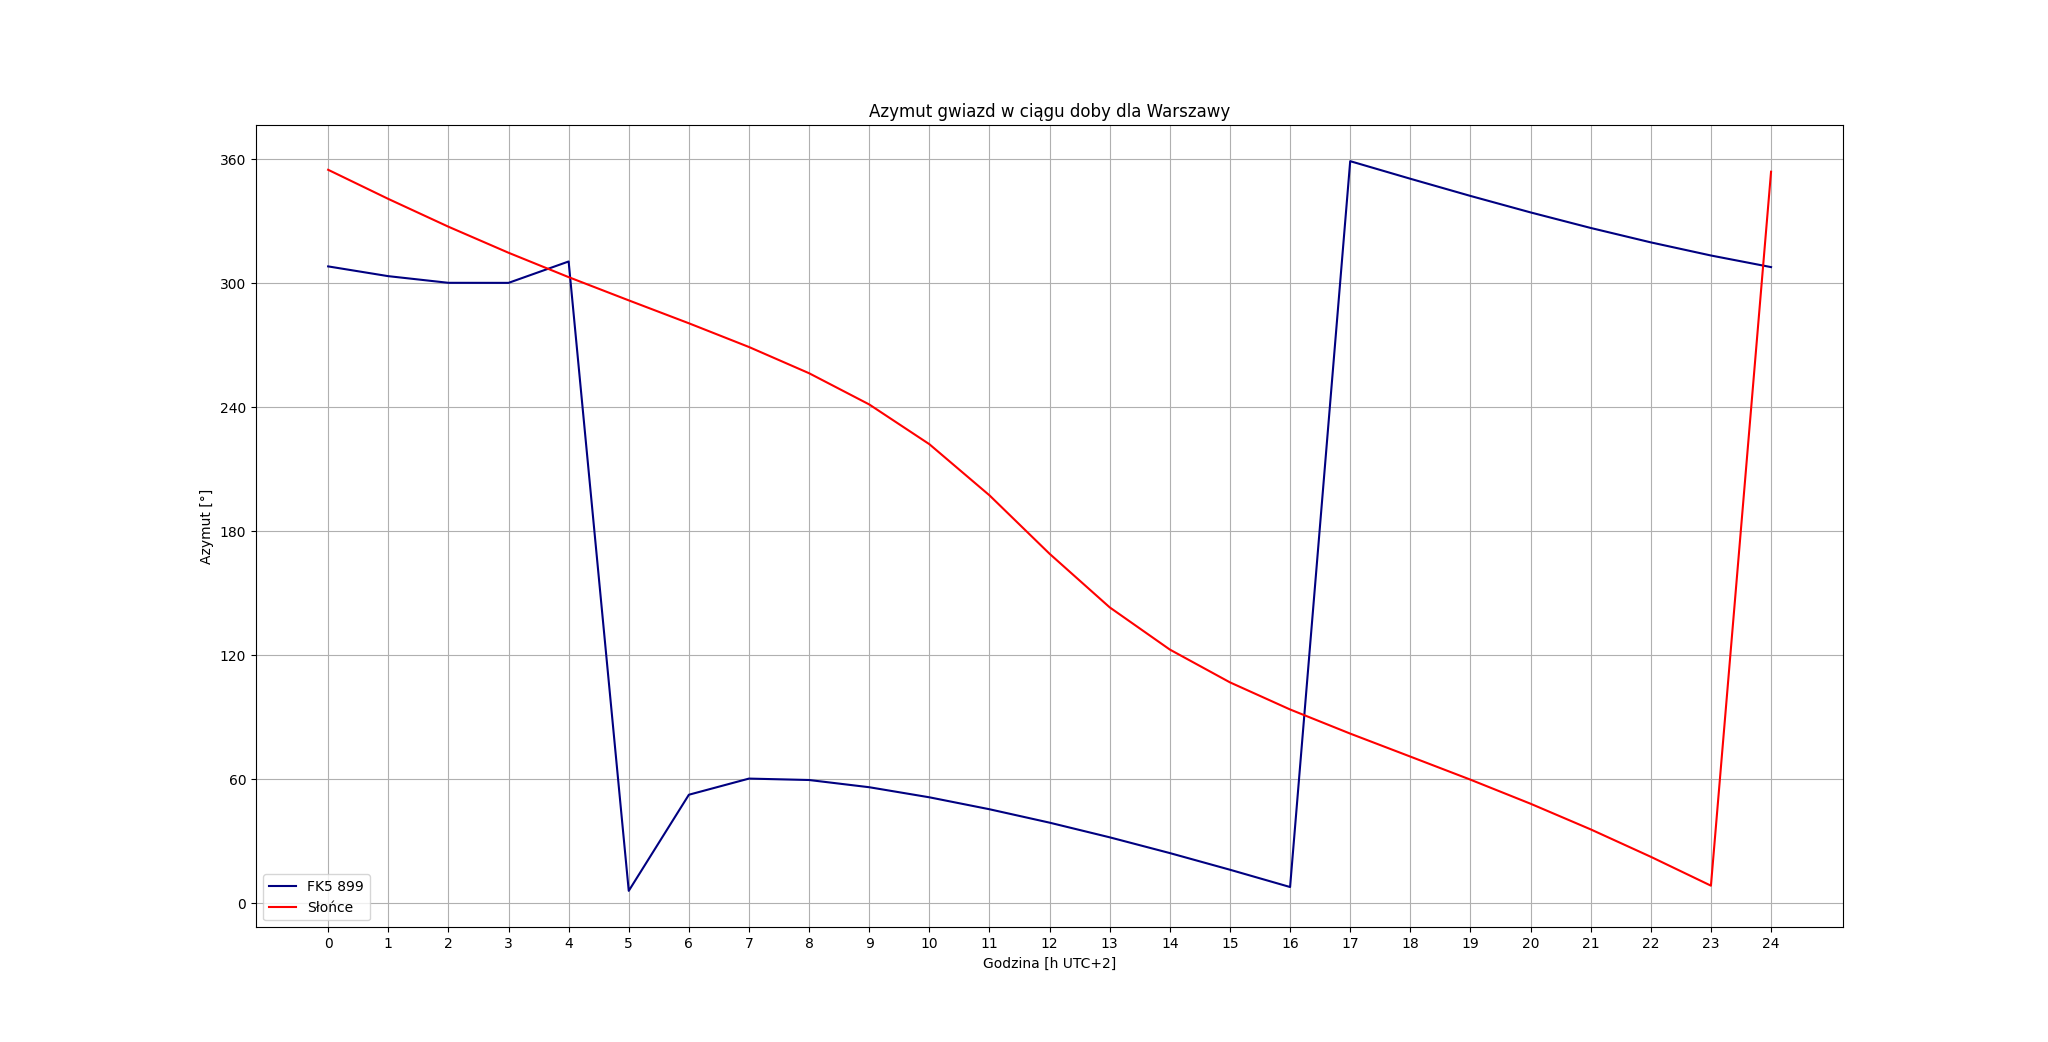
\includegraphics[width=1\textwidth]{zdjecia/az_gwiazd_wwa.png}
  \caption{Wykres azymutu gwiazd od godziny z punktu obserwacji Warszawa}
  \label{az_wwa}
\end{figure}
Przełamania na wykresie \ref{az_wwa} odpowiadają godzinom, w których gwiazdy osiągają najmniejszą oraz największą wysokość.
Są one spowodoowane tym, że gwiazdy przechodzą przez punkt północy i zmieniają swoją wartość z 360° na 0°.

\clearpage
\begin{figure}[h!]
  \centering
  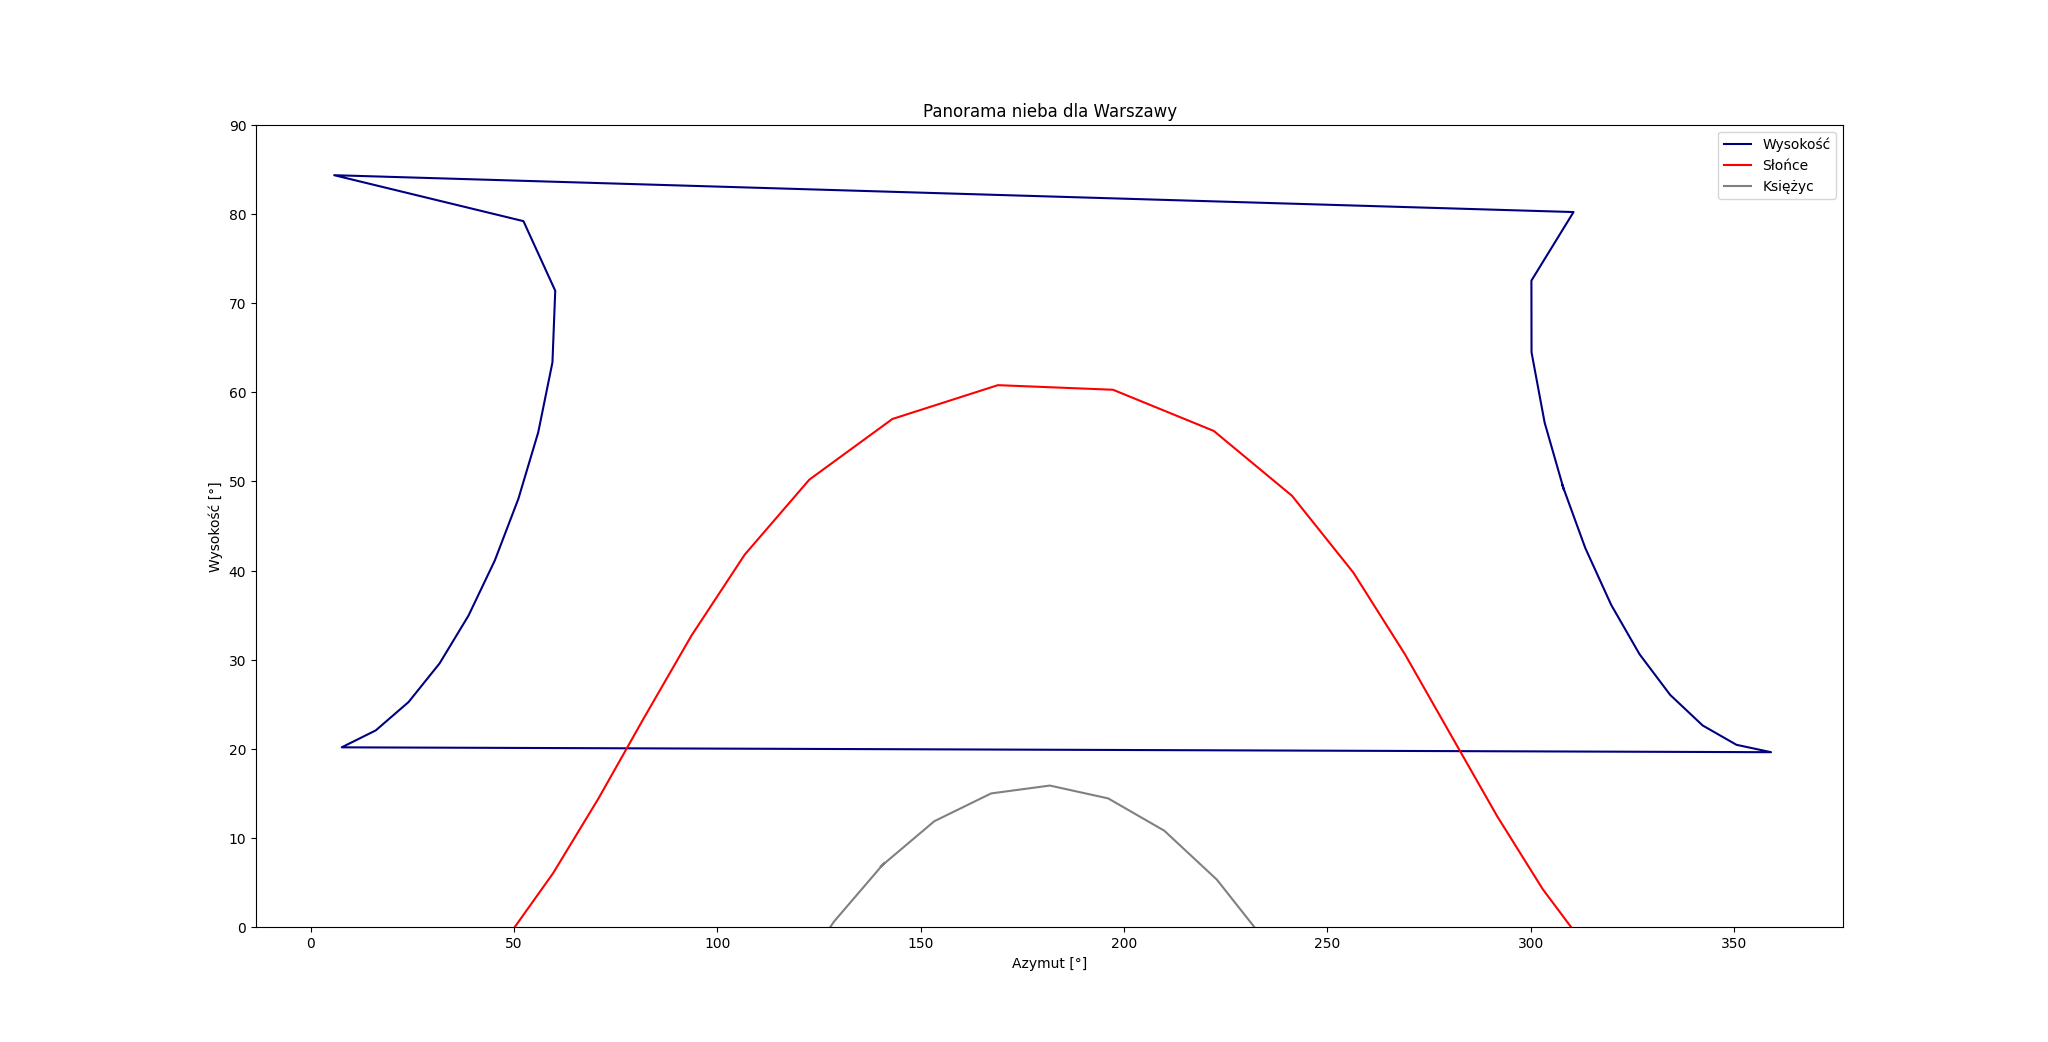
\includegraphics[width=1\textwidth]{zdjecia/panorama_wwa_b.png}
  \caption{Panorama nieba z punktu obserwacji Warszawa}
  \label{pan_wwa}
\end{figure}

\subsection{Wielki Wóz}

\begin{figure}[h!]
  \centering
  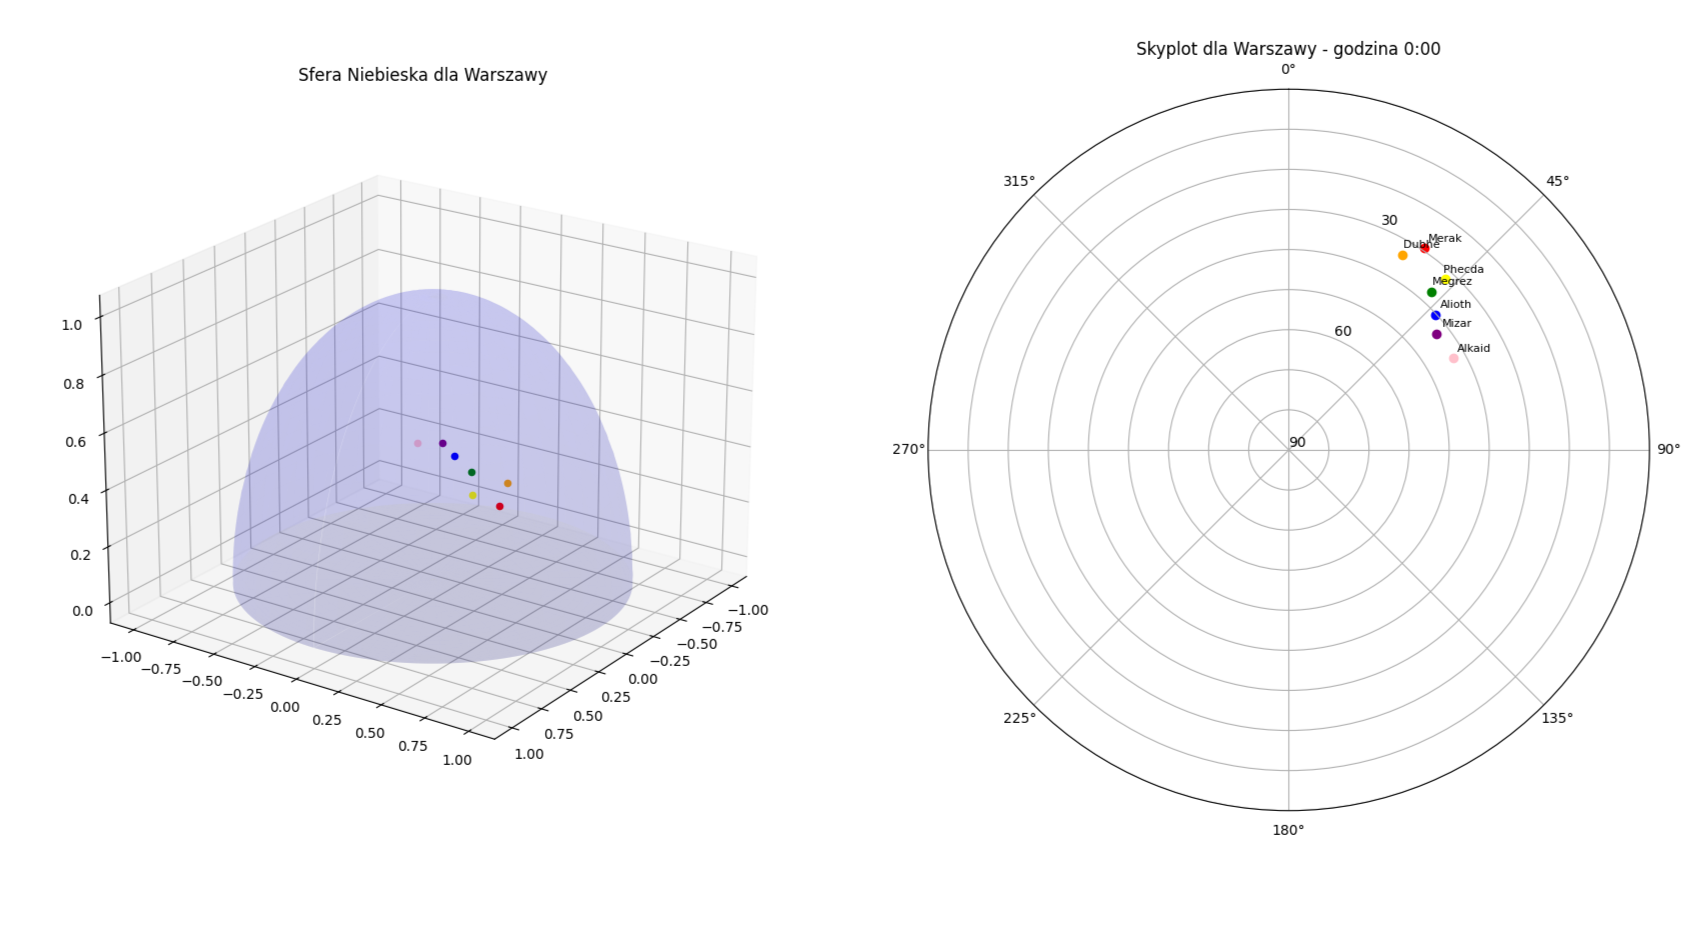
\includegraphics[width=1\textwidth]{zdjecia/wielkiwoz1_wwa.png}
  \caption{Położenie gwiazd Wielkiego Wozu o godzinie 0:00 z punktu obserwacji Warszawa}
  \label{wielkiwoz_wwa_0}
\end{figure}

Wykres \ref{wielkiwoz_wwa_0} obrazuje położenie gwiazd o godzinie 0:00.
Ta reprezentacja pokazuje z nam charakterystyczny kształt Wielkiego Wozu, którego można się spodziewać.

Załączony do sprawozdania Kod źródłowy \ref{kod4} służy do animacji cogodzinnego położenia 
gwiazd Wielkiego Wozu na sferze niebieskiej. 
Jej efekty przedstawiają filmy \texttt{wielkiwoz\_warszawa.mp4} oraz \texttt{wielkiwoz\_rownik.mp4}, które zawierają animację odpowiednio
z Warszawy i Równika. 
Pomimo, że położenia poszczególnych gwiazd się zmieniają, kształt Wielkiego Wozu pozostaje niezmienny oraz widoczny z Warszawy przez całą dobę. 
Można spostrzec, że gwiazda Alkaid jako jedyna przechodzi przez Pierwszy Wertykał o godzinie 18:00 oraz 21:00.

\begin{figure}[h!]
  \centering
  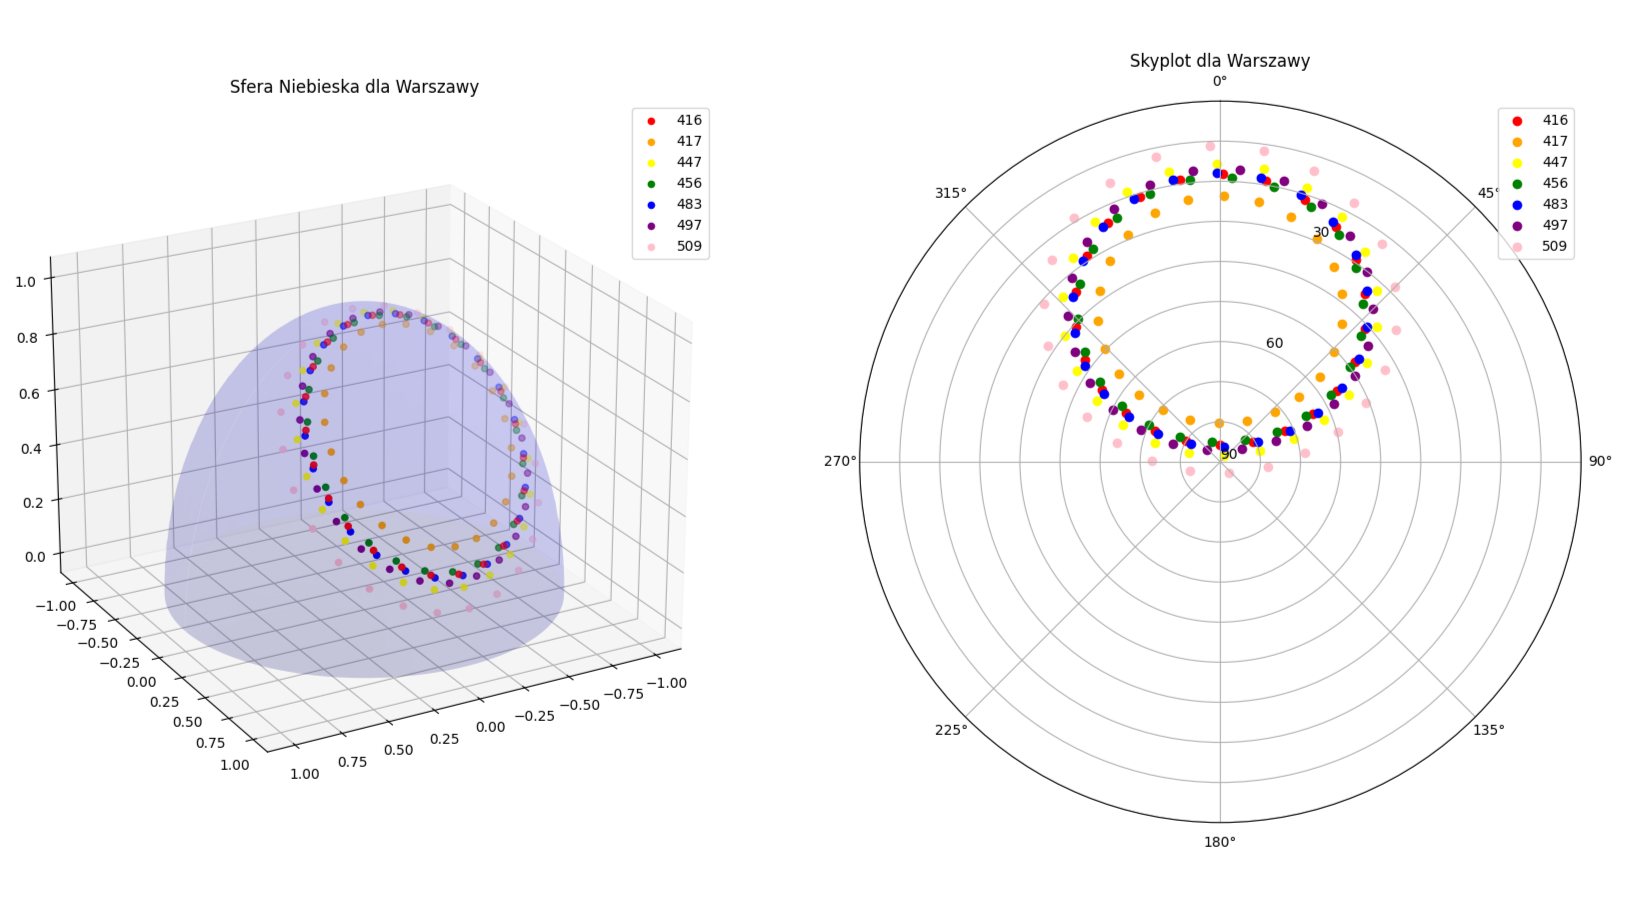
\includegraphics[width=1\textwidth]{zdjecia/wielkiwoz_wwa.png}
  \caption{Położenie gwiazd Wielkiego Wozu w ciągu doby z punktu obserwacji Warszawa}
  \label{wielkiwoz_wwa}
\end{figure}


Wizualizacja całodobowa na wykresie \ref{wielkiwoz_wwa} potwierdza, że gwiazdy Wielkiego Wozu są w Warszawie widoczne przez całą dobę.

\section{Równik}
\subsection{Ro Cassiopeiae i Słońce}

\begin{figure}[h!]
    \centering
    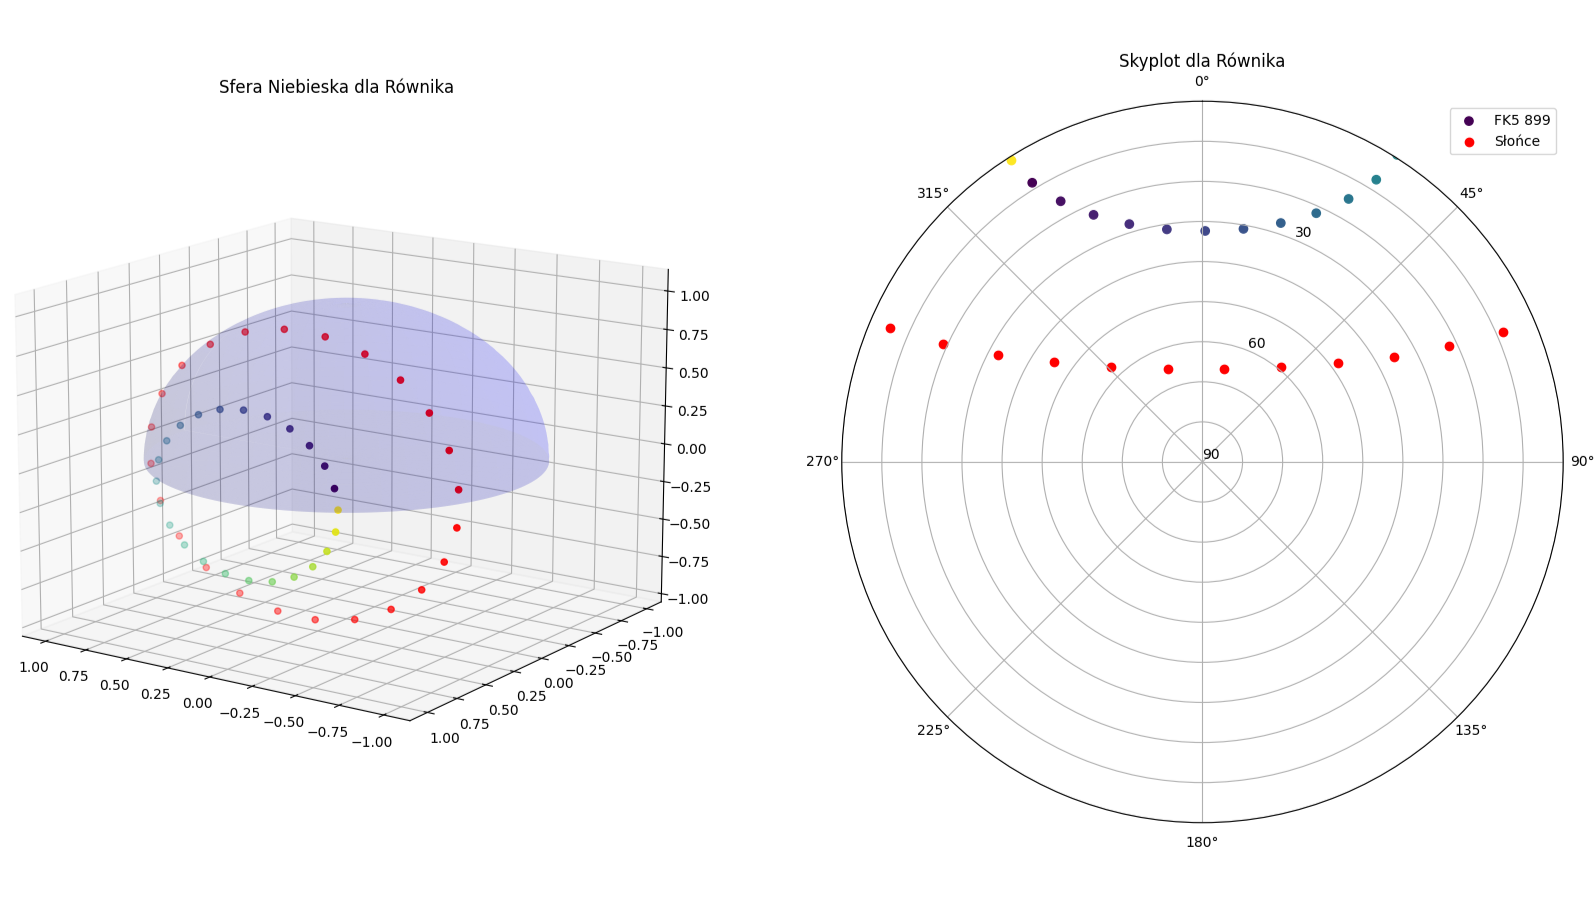
\includegraphics[width=0.99\textwidth]{zdjecia/fig1_r.png}
    \caption{Położenia gwiazd w ciągu doby z punktu obserwacji Równik}
    \label{all_r}
\end{figure}

\begin{figure}[h!]
  \centering
  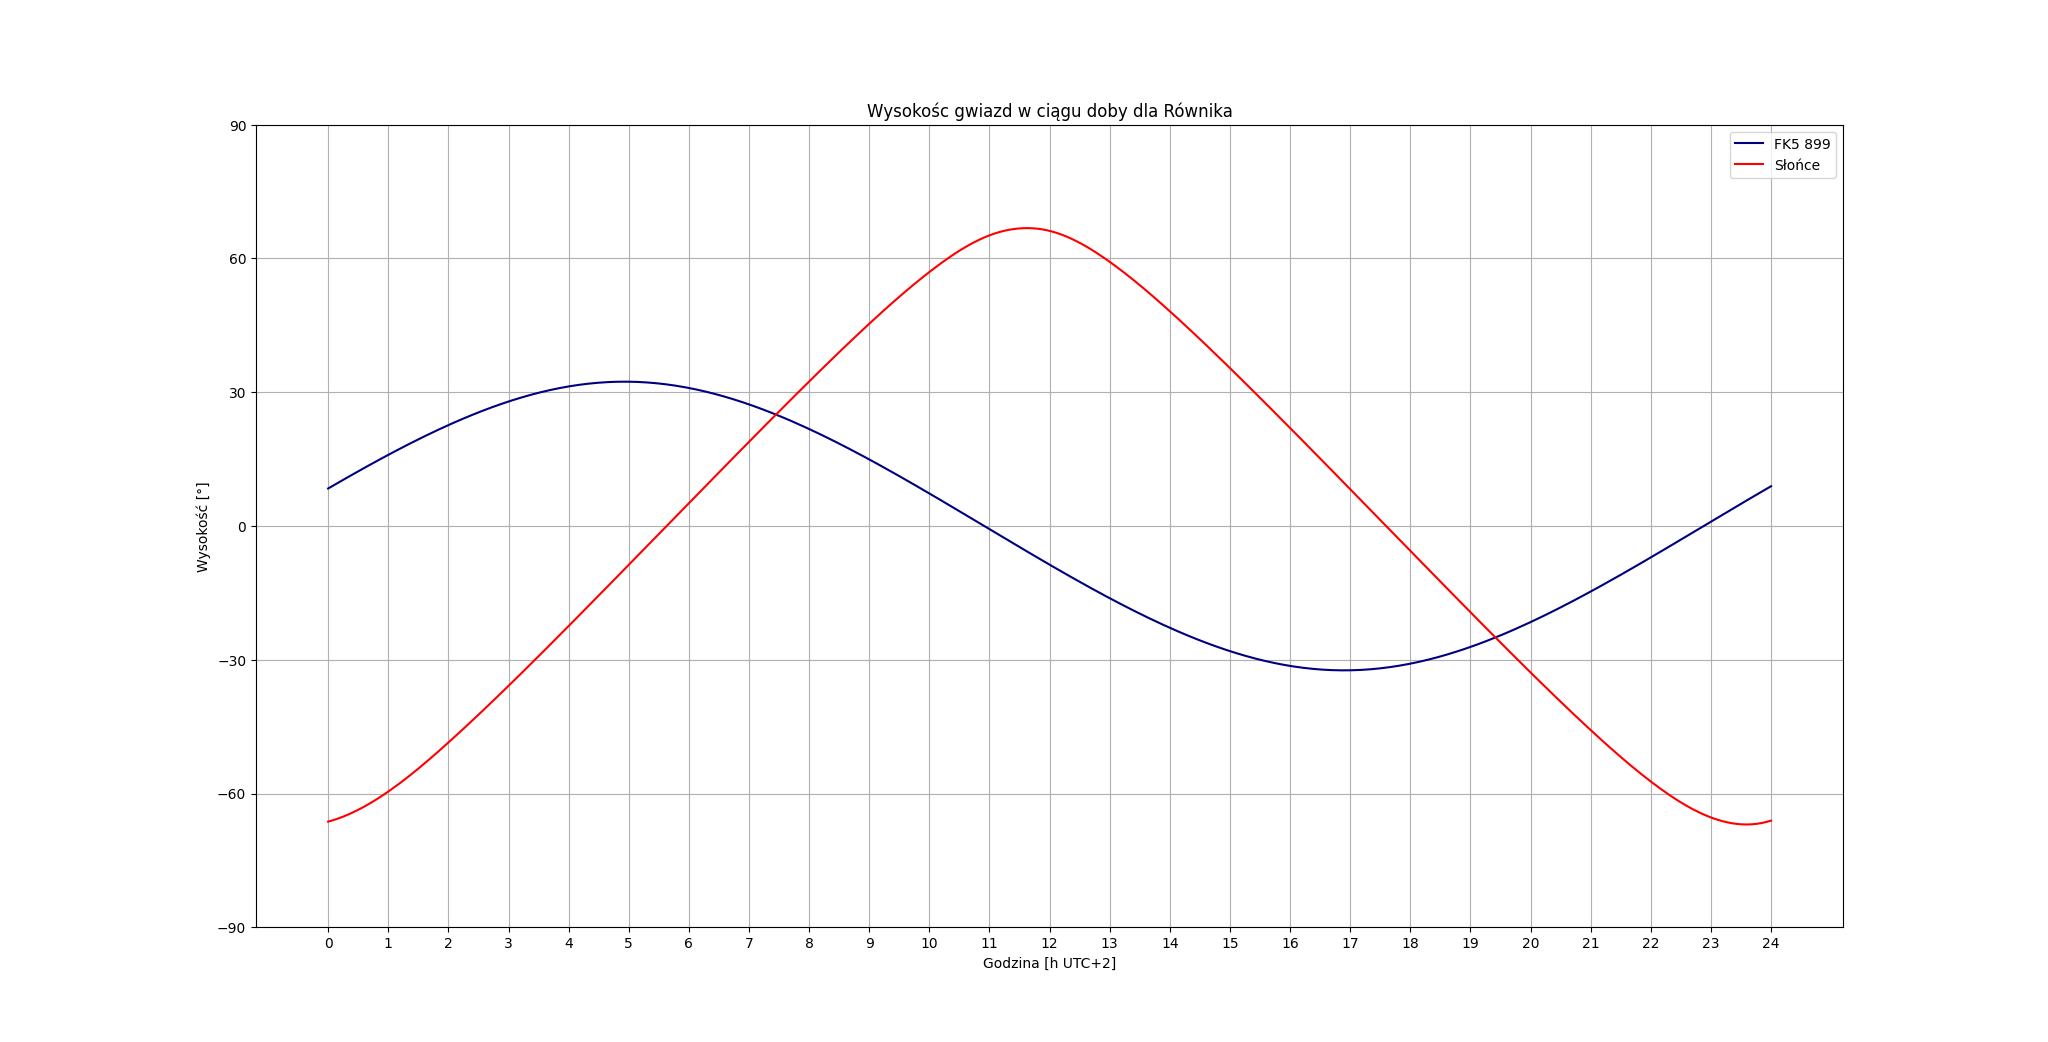
\includegraphics[width=1\textwidth]{zdjecia/wys_gwiazd_r_inter.png}
  \caption{Wykres wysokości gwiazd od godziny z punktu obserwacji Równik}
  \label{h_r}
\end{figure}

\begin{figure}[h!]
  \centering
  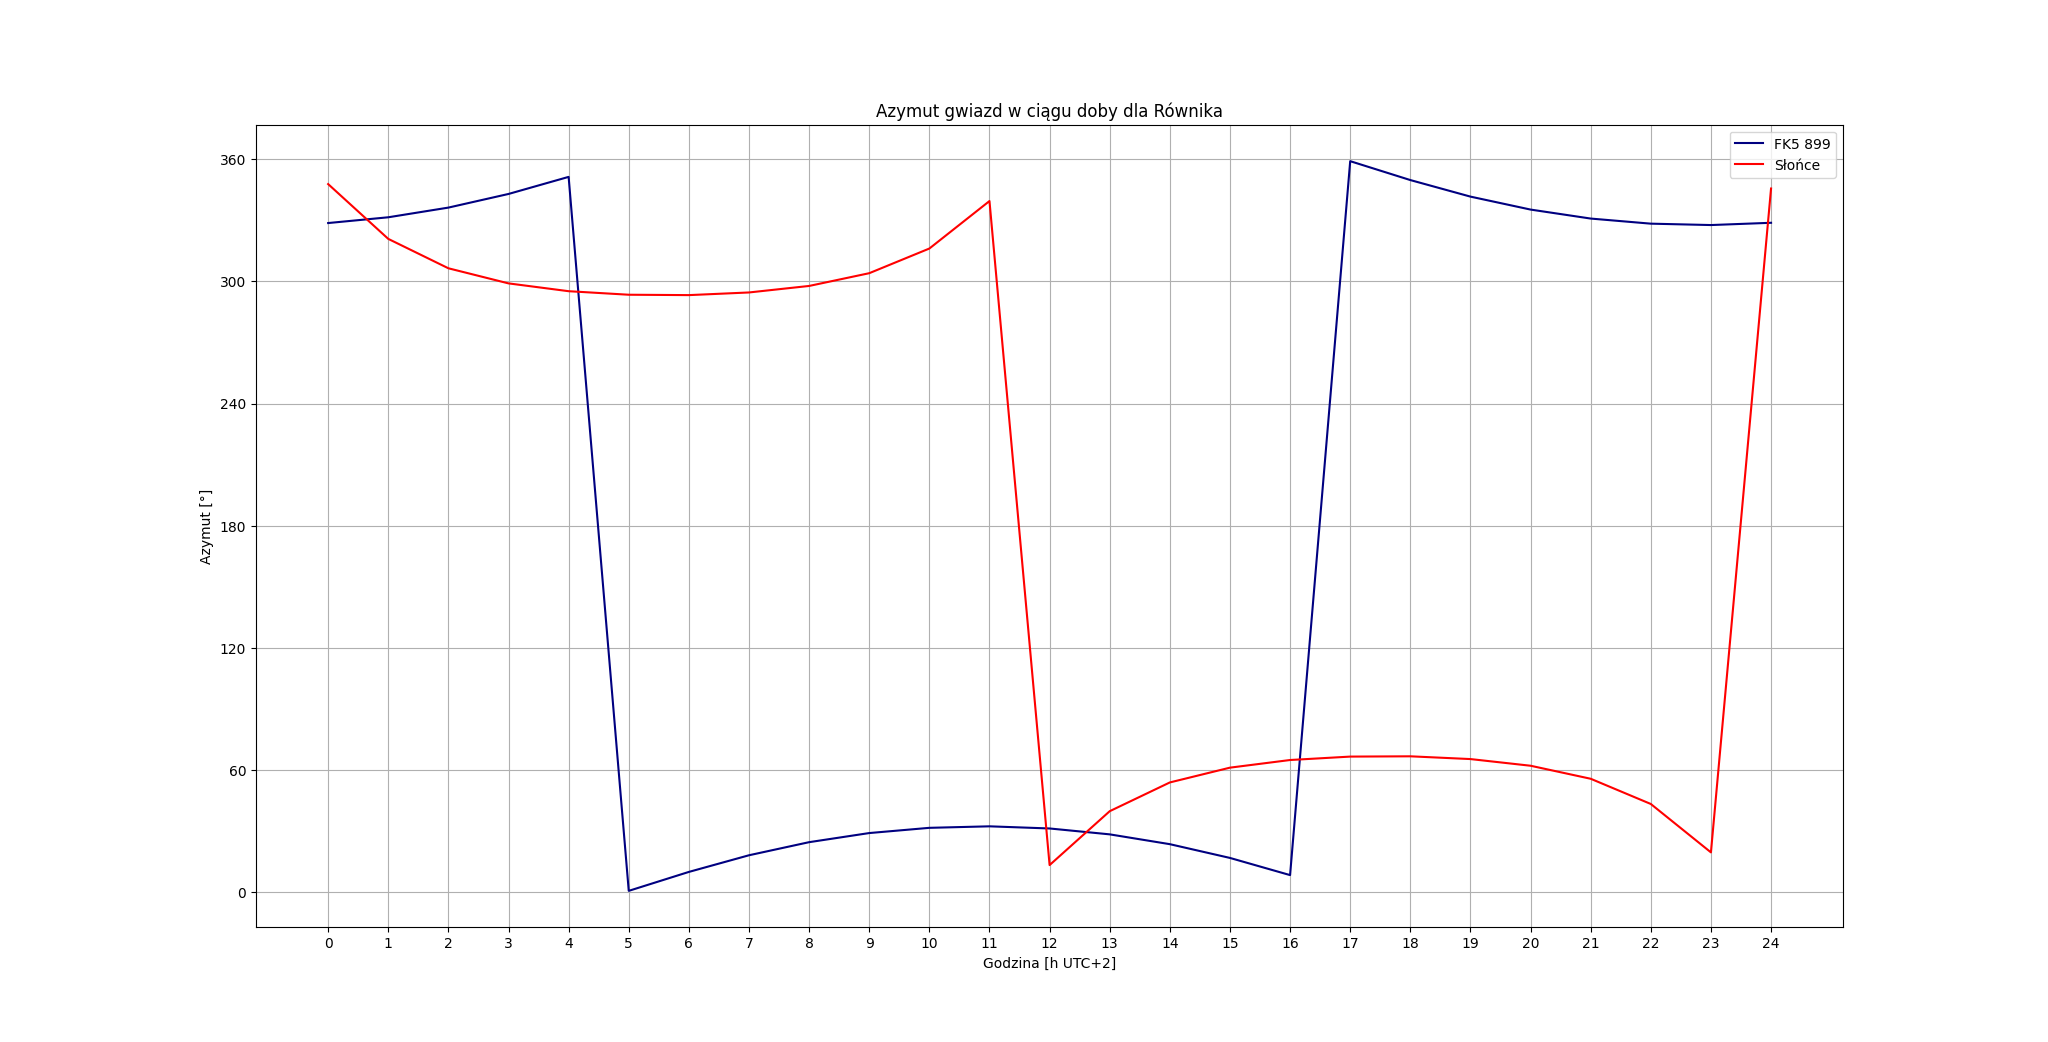
\includegraphics[width=1\textwidth]{zdjecia/az_gwiazd_r.png}
  \caption{Wykres azymutu gwiazd od godziny z punktu obserwacji Równik}
  \label{az_r}
\end{figure}

Na wykresie \ref{h_r} gwiazdy możemy zauważyć, 
że Ro Cassiopeiae zachodzi około godziny 11:00 i nie jest widoczna aż do 23:00. Jej górowanie przypada na godzinę 5:00,
tak samo jak w przypadku Warszawy.

Słońce na Równiku w tym dniu widoczne jest około 12h. Góruje wysoko nad horyzontem przed godziną 12:00, i osiąga wysokość ponad 60°.
Jego wykres jest symetryczny względem godzin południowych.

\newpage
\begin{figure}[h!]
  \centering
  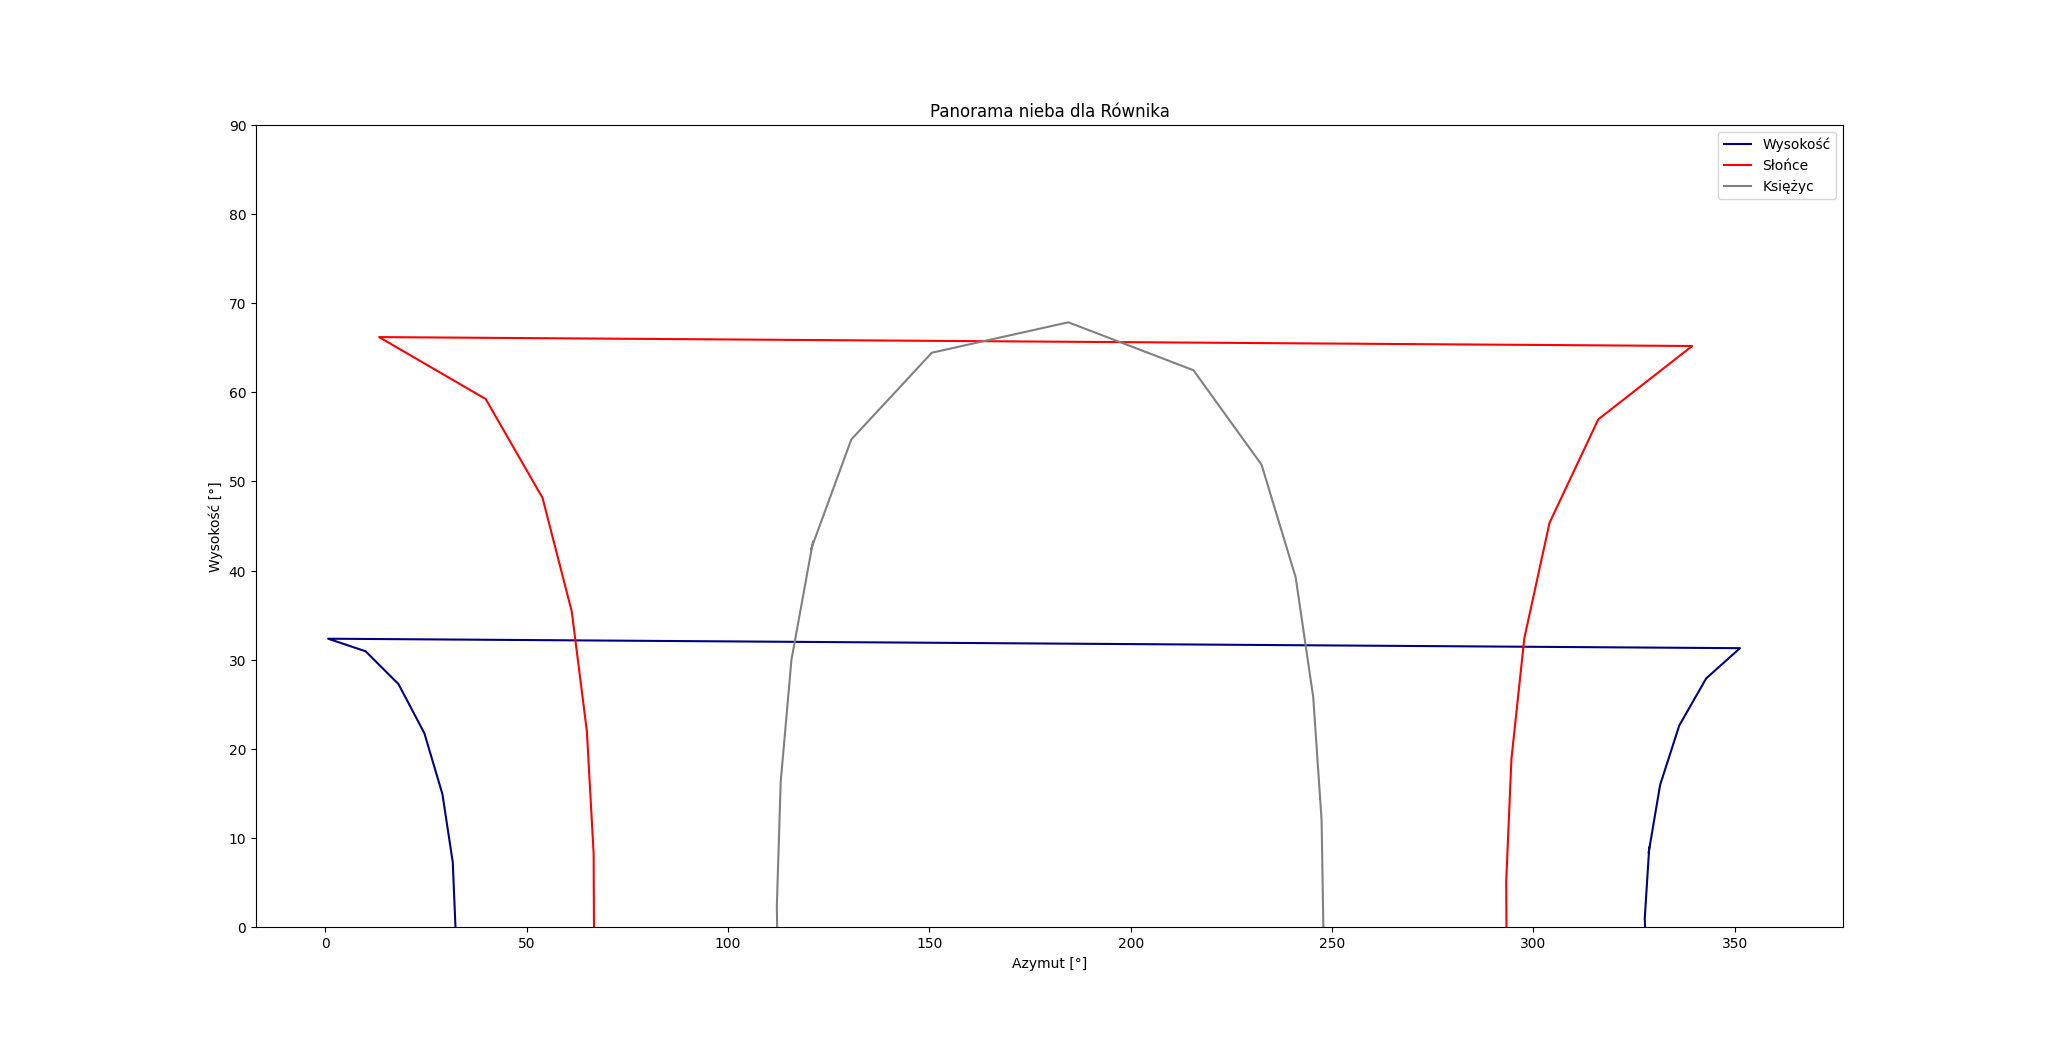
\includegraphics[width=1\textwidth]{zdjecia/panorama_r_b.png}
  \caption{Panorama nieba z punktu obserwacji Równik}
  \label{zjdecia/panorama_r}
\end{figure}
\clearpage
\newpage
\subsection{Wielki Wóz}

\begin{figure}[h!]
  \centering
  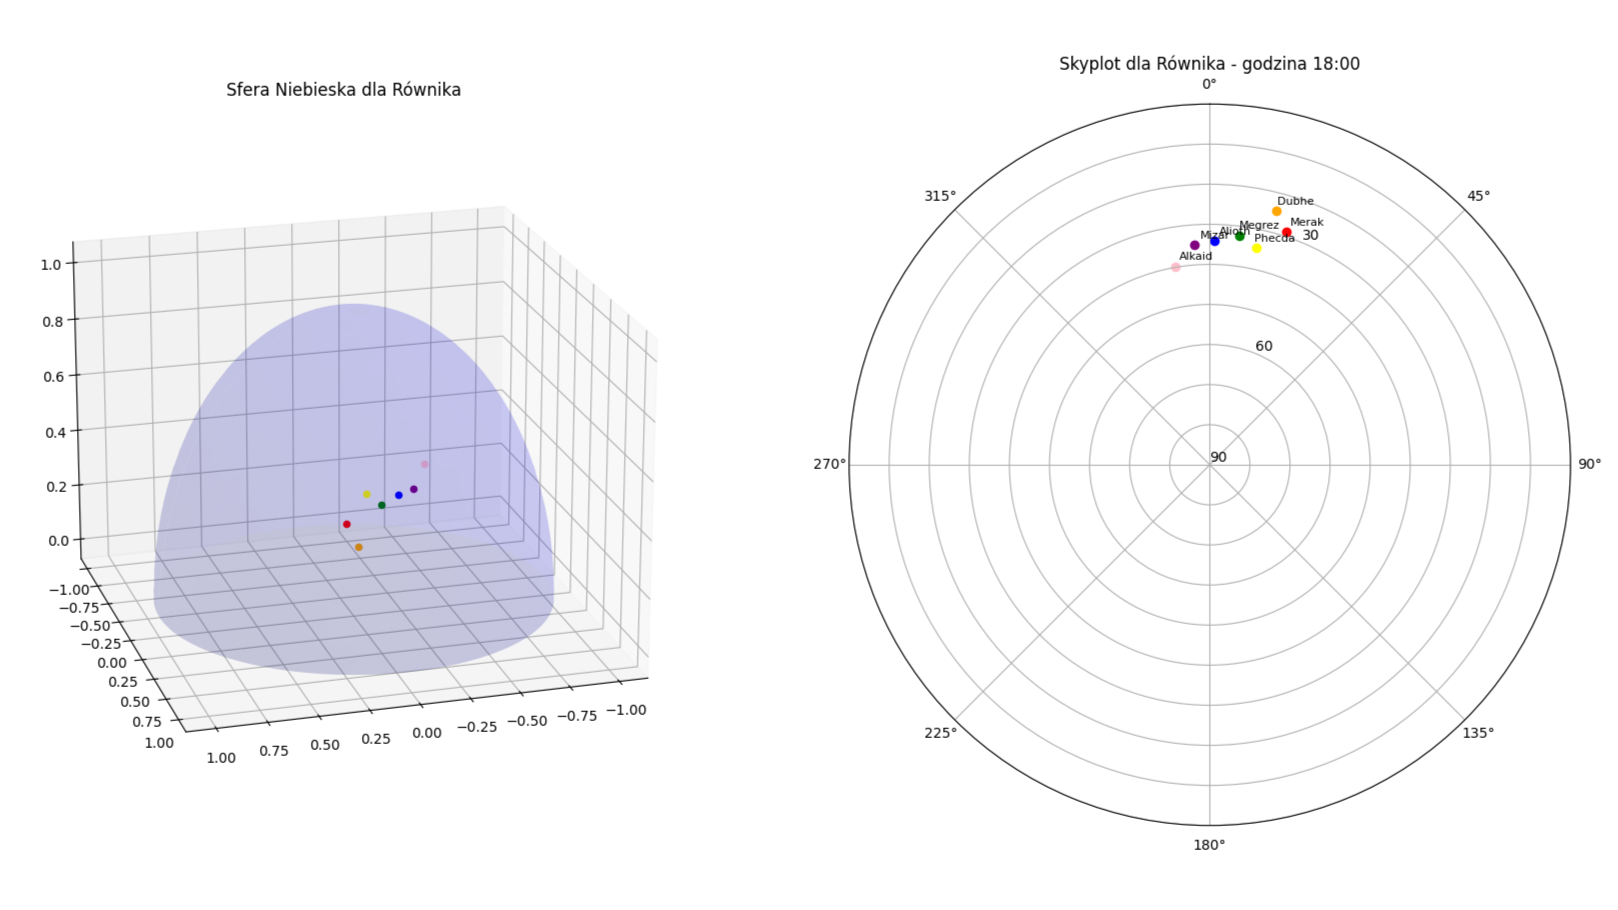
\includegraphics[width=1\textwidth]{zdjecia/wielkiwoz18_r.png}
  \caption{Położenie Wielkiego Wozu o godzinie 18:00 z punktu obserwacji Równik}
  \label{wielkiwoz_r18}
\end{figure}

\begin{figure}[h!]
  \centering
  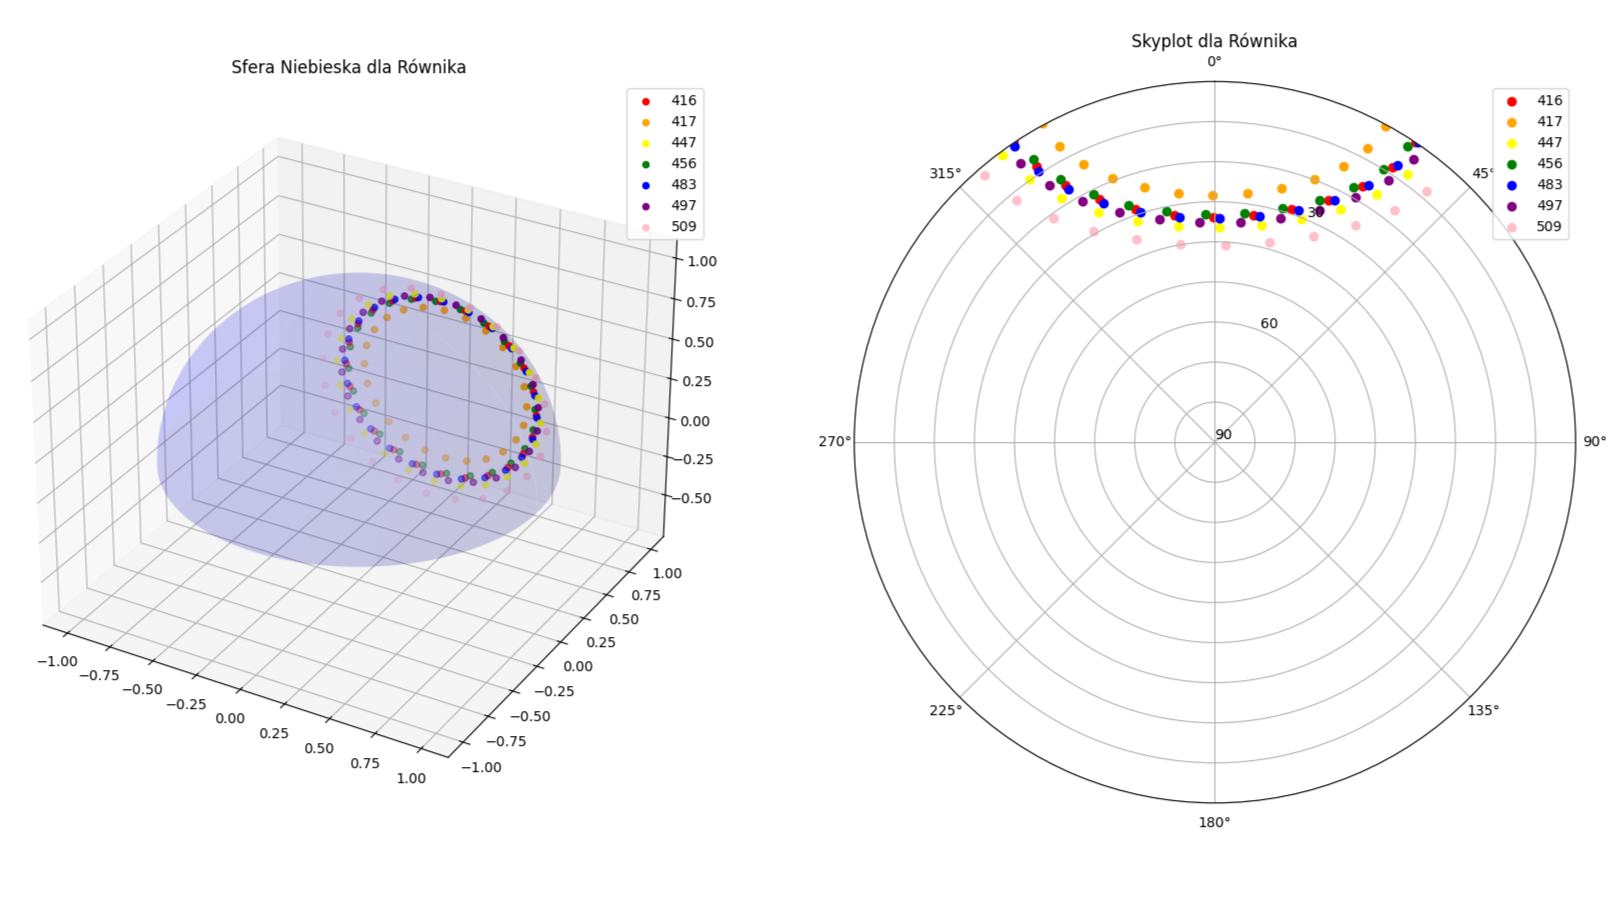
\includegraphics[width=1\textwidth]{zdjecia/wielkiwoz_r.png}
  \caption{Położenie Wielkiego Wozu w ciągu doby z punktu obserwacji Równik}
  \label{wielkiwoz_r}
\end{figure}

Z punktu widzenia obserwatora na Równiku, wszystkie gwiazdy Wielkiego Wozu wschodzą i zachodzą. Są widoczne
przez około 13h, a ich położenie na sferze niebieskiej jest podobne do analizowanej gwiazdy FK5 899.

\clearpage
\newpage

\section{Kod programu}

\begin{lstlisting}[language=Python, caption=Funkcje udostępnione przez prowadzącego, label = kod1]
  def dms2deg(dms):
      d = dms[0]
      m = dms[1]
      s = dms[2]
      
      deg = d+m/60+s/3600
      return deg
  
  def dms2rad(dms):
      d = dms[0]
      m = dms[1]
      s = dms[2]
      
      deg = d+m/60+s/3600
      rad = np.deg2rad(deg)
      return rad
  
  def julday(y, m, d, h):
      if m <= 2:
          y = y - 1
          m = m + 12
      jd = np.floor(365.25*(y+4716))+np.floor(30.6001*(m+1))+d+h/24-1537.5
      return jd
  
  def GMST(jd):
      T = (jd - 2451545) / 36525
      Tu = jd - 2451545
      g = 280.46061837 + 360.98564736629*(jd - 2451545.0) + 0.000387933*T**2-T**3/38710000
      g = (g%360) / 15
      return g
\end{lstlisting}
\newpage
\begin{lstlisting}[language=Python, caption=Funkcje własne, label = kod2]
  def horizontal_coords(alpha, delta, phi, L, gmst):
      H = (gmst * 15 + L - alpha * 15) % 360
      H = np.radians(H)
      phi = np.radians(phi)
      delta = np.radians(delta)
  
      h = np.arcsin(np.sin(delta)*np.sin(phi) + np.cos(delta)*np.cos(phi)*np.cos(H))
      A = np.arccos((np.sin(delta) - np.sin(phi)*np.sin(h)) / (np.cos(phi)*np.cos(h)))
  
      h = np.degrees(h)
      A = np.degrees(A)
  
      H = np.degrees(H)
      A = np.where(H > 180, 360 - A, A)
  
      return h, A
  
  def interpolate(hours, h_values, label, color):
      xnew = np.linspace(min(hours), max(hours), 300)
      spl = make_interp_spline(hours, h_values, k=3)
      ynew = spl(xnew)
      # plt.fill_between(xnew, 0, ynew, where=(ynew > 0), color=color, alpha=1, label = label)
  
\end{lstlisting}
\newpage
\begin{lstlisting}[language=Python, caption=Implementacja wykresów położenia gwiazdy FK5 899, label = kod3]
  # Współrzędne gwiazd
  alpha_hms = [23, 55, 34.219]
  delta_hms = [57, 37, 48.71]
  alpha = dms2deg(alpha_hms)
  delta = dms2deg(delta_hms)
  
  # Słońce
  alpha_s = dms2deg([6, 37, 43.973])
  delta_s = dms2deg([23, 8, 11.85])
  
  # Współrzędne obserwatorów
  locations = {
      'Warszawy': {'phi': 52, 'L': 21},
      'Równika': {'phi': 0, 'L': 21},
  }
  
  if __name__ == '__main__':
  # Tworzenie wykresów
      for location, coords in locations.items():
          phi = coords['phi']
          L = coords['L']
  
          # Obliczanie lokalnych współrzędnych horyzontalnych co godzinę
          hours = np.arange(0, 25, 1)
          h_values = []
          A_values = []

          # Te same obliczenia zostały wykonane dla Słońca i Księżyca
          for hour in hours:
              jd = julday(2023, 7, 1, hour - 1)  # UTC+2 dla Polski
              gmst = GMST(jd)
              h, A = horizontal_coords(alpha, delta, phi, L, gmst)
              h_values.append(h)
              A_values.append(A)

          h_values = np.array(h_values)
          A_values = np.array(A_values)

          # Sfera Niebieska
          fig = plt.figure(figsize=(10, 10))
          ax = fig.add_subplot(121, projection='3d')
          u, v = np.mgrid[0:(2 * np.pi):0.01, 0:np.pi:0.01]
          x = np.cos(u) * np.sin(v)
          y = np.sin(u) * np.sin(v)
          z = np.cos(v)
          z[z < 0] = 0
          ax.plot_surface(x, y, z, alpha=0.1, color='b')
          gx = np.sin(np.radians(A_values)) * np.cos(np.radians(h_values))
          gy = np.cos(np.radians(A_values)) * np.cos(np.radians(h_values))
          gz = np.sin(np.radians(h_values))
          ax.scatter(gx, gy, gz, c=hours, cmap='viridis', label = 'FK5 899')
  
          ax.set_title(f'Sfera Niebieska dla {location}')
  
          # Skyplot
          ax = plt.subplot(122, polar=True)
          ax.set_theta_zero_location('N')
          ax.set_theta_direction(-1)
          ax.set_yticks(range(0, 90+10, 10))
          yLabel = ['90', '', '', '60', '', '', '30', '', '', '']
          ax.set_yticklabels(yLabel)
          ax.set_rlim(0, 90)
          ax.scatter(np.radians(A_values), 90 - h_values, c=hours, cmap='viridis', label = 'FK5 899')
          ax.set_title(f'Skyplot dla {location}')
          ax.legend()
  
          # Wykresy zależności wysokości i azymutu od czasu
          # Azymut
          plt.figure(figsize=(10, 5))
          plt.plot(hours, A_values, label='FK5 899', color = 'navy')
          plt.xticks(range(25))
          plt.xlabel('Godzina [h UTC+2]')
          plt.ylabel('Azymut [\degree]')
          plt.yticks(np.arange(0, 361, 60))
          plt.legend()
          plt.grid()
          plt.title(f'Azymut gwiazd w ciągu doby dla {location}')
          
          # Wysokość
          plt.figure(figsize=(10, 5))
          plt.plot(hours, h_values, label='FK5 899', color = 'navy')
          plt.xticks(range(25))
          plt.yticks(np.arange(-90, 91, 30))
          plt.xlabel('Godzina [h UTC+2]')
          plt.ylabel('Wysokość [\degree]')
          plt.legend()
          plt.grid()
          plt.title(f'Wysokośc gwiazd w ciągu doby dla {location}')
          
          # Panorama
          plt.figure(figsize=(10, 5))
          plt.plot(A_values, h_values, label = 'Wysokość', color = 'navy')
          plt.ylim(0, 90)
          plt.title(f'Panorama nieba dla {location}')
          plt.xlabel('Azymut [\degree]')
          plt.ylabel('Wysokość [\degree]')
          plt.legend()
          
          plt.show()
\end{lstlisting}
\newpage
\begin{lstlisting}[language=Python, caption=Animacja położenia gwiazd Wielkiego Wozu, label = kod4]
# Współrzędne gwiazd
FK5 = {
    'Merak' : {'alpha' : [11, 3, 14.669], 'delta' : [56, 15, 21.18]}, #416
    'Dubhe ' : {'alpha' : [11, 5, 9.530], 'delta' : [61, 37, 24.44]}, #417
    'Phecda ' : {'alpha' : [11, 55, 3.388], 'delta' : [53, 33, 50.55]}, #447
    'Megrez' : {'alpha' : [12, 16, 34.755], 'delta' : [56, 54, 7.8]}, #456
    'Alioth' : {'alpha' : [12, 55, 3.395], 'delta' : [55, 49, 57.62]}, #483
    'Mizar' : {'alpha' : [13, 24, 52.075], 'delta' : [54, 48, 11.5]}, #497
    'Alkaid' : {'alpha' : [13, 48, 27.861], 'delta' : [49, 11, 48.04]}, #509
}

colors = ['red', 'orange', 'yellow', 'green', 'blue', 'purple', 'pink']
color_index = 0

# Współrzędne obserwatorów
locations = {
    'Warszawy': {'phi': 52, 'L': 21},
    'Równika': {'phi': 0, 'L': 21},
}

for location, coords in locations.items():
    # Sfera Niebieska
    fig = plt.figure(figsize=(10, 10))
    ax = fig.add_subplot(121, projection='3d')
    u, v = np.mgrid[0:(2 * np.pi):0.01, 0:np.pi:0.01]
    x = np.cos(u) * np.sin(v)
    y = np.sin(u) * np.sin(v)
    z = np.cos(v)
    z[z < 0] = 0
    ax.plot_surface(x, y, z, alpha=0.1, color='b')

    # Skyplot
    ax2 = plt.subplot(122, polar=True)
    ax2.set_theta_zero_location('N')
    ax2.set_theta_direction(-1)
    ax2.set_yticks(range(0, 90+10, 10))
    yLabel = ['90', '', '', '60', '', '', '30', '', '', '']
    ax2.set_yticklabels(yLabel)
    ax2.set_rlim(0, 90)

    color_index = 0
    phi = coords['phi']
    L = coords['L']

    ax.set_title(f'Sfera Niebieska dla {location}')
    ax2.set_title(f'Skyplot dla {location}')
    
    lines_sfera = []
    lines_skyplot = []
    
    # Pobranie danych o gwiazdach
    for star_name, star_coords in FK5.items():
        alpha = dms2deg(star_coords['alpha'])
        delta = dms2deg(star_coords['delta'])
        color = colors[color_index]
        
        line_sfera, = ax.plot([], [], 'o-', color=color, label=star_name)
        line_skyplot, = ax2.plot([], [], 'o-', color=color, label=star_name)
        
        lines_sfera.append(line_sfera)
        lines_skyplot.append(line_skyplot)
        
        color_index = (color_index + 1) % len(colors)
        
    ax.legend(loc = 'upper right')
    ax2.legend(loc = 'upper right')
    
    # Obliczanie lokalnych współrzędnych horyzontalnych co godzinę
    for hour in np.arange(0, 24, 1):
        h_values_all = []
        A_values_all = []
        gx_all = []
        gy_all = []
        gz_all = []
        
        for star_coords in FK5.values():
            h_values = []
            A_values = []
            alpha = dms2deg(star_coords['alpha'])
            delta = dms2deg(star_coords['delta'])
            
            jd = julday(2023, 7, 1, hour - 1) 
            gmst = GMST(jd)
            h, A = horizontal_coords(alpha, delta, phi, L, gmst)
            h_values.append(h)
            A_values.append(A)

            h_values = np.array(h_values)
            A_values = np.array(A_values)
                
            gx = np.sin(np.radians(A_values)) * np.cos(np.radians(h_values))
            gy = np.cos(np.radians(A_values)) * np.cos(np.radians(h_values))
            gz = np.sin(np.radians(h_values))
            
            gx_all.append(gx)
            gy_all.append(gy)
            gz_all.append(gz)
            h_values_all.append(h_values)
            A_values_all.append(A_values)
            
        # Zaktualizowanie danych na wykresach
        for i in range(len(FK5)):
            lines_sfera[i].set_data(gx_all[i], gy_all[i])
            lines_sfera[i].set_3d_properties(gz_all[i])
            lines_skyplot[i].set_data(np.radians(A_values_all[i]), 90 - h_values_all[i])
        
        plt.draw()
        plt.pause(0.5)

plt.show()
\end{lstlisting}

\listoftables
\listoffigures
\lstlistoflistings

\end{document}